\documentclass{standalone}
\usepackage{tikz,amsmath}
\usetikzlibrary{shapes.geometric}
\tikzset{block/.style = {draw, fill=white, very thick, rectangle, minimum height=1cm, minimum width=2cm},}
\tikzset{sum/.style= {draw, fill=white, very thick, circle, node distance=1cm},}
\tikzset{triangle/.style= {draw, fill=white, very thick, isosceles triangle, minimum height=2cm, minimum width=1cm},}
\begin{document}
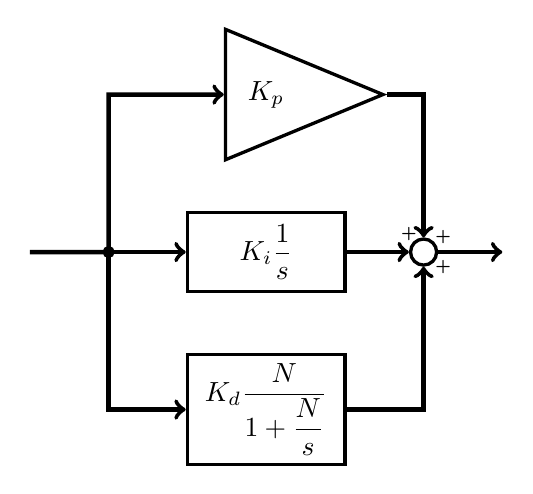
\begin{tikzpicture}[scale=2]
    \node[triangle](p)at(0,1){$K_p$};
    \node[block](i)at(0,0){$\displaystyle K_i\frac{1}{s}$};
    \node[block](d)at(0,-1){$\displaystyle K_d\frac{N}{1+\displaystyle\frac{N}{s}}$};

    \draw[->,ultra thick](-1.5,0)--(-1,0)--(-1,1)--(p.180);
    \draw[->,ultra thick](-1,0)--(i.180);
    \draw[->,ultra thick](-1,0)--(-1,-1)--(d.180);
    \filldraw[black](-1,0)circle(1pt);
    \node[sum](s)at(1,0){};

    \draw[->,ultra thick](p.0)--(1,1)--(s.90)node[right]{$\scriptscriptstyle\boldsymbol{+}$};
    \draw[->,ultra thick](i.0)--(s.180)node[above]{$\scriptscriptstyle\boldsymbol{+}$};
    \draw[->,ultra thick](d.0)--(1,-1)--(s.270)node[right]{$\scriptscriptstyle\boldsymbol{+}$};
    \draw[->,ultra thick](s.0)--(1.5,0);
\end{tikzpicture}
\end{document}